\chapter{Contracts}
\label{ch:contracts}

\newcommand{\lecnum}{1}
%\newcommand{\lectitle}{Contracts}
\newcommand{\lecturer}{Frank Pfenning, Iliano Cervesato}

\chapterTAGS{correctness, interpreter, loop-invariant, safety, testing}
\maketitle

\begin{preamble}
\noindent
In these notes we review \emph{contracts}, which we use to
collectively denote function contracts, loop invariants, and other
assertions about a program.  Contracts will play a central role in
this class, since they represent the key to connect algorithmic ideas
to imperative programs.  We do this through an example, developing
annotations for a given program that express the contracts, thereby
making the program understandable (and allowing us to find a bug).
\end{preamble}

\begin{gram}[Learing Goals]
In term of our learning goals, this lecture addresses:
\begin{description}
\item[Computational Thinking:]

  Developing contracts (preconditions, postconditions, assertions, and
  loop invariants) that establish the safety and correctness of
  imperative programs.

  Using point-to reasoning to develop proofs of the safety and
  correctness of code with contracts.

  Developing informal termination arguments for
  programs with loops and recursion.

  Identifying the difference between \emph{specification} and
  \emph{implementation}.
\item[Algorithms and Data Structures:]
  Integer algorithms (fast power).
\item[Programming:] Identifying, describing, and effectively using
  \lstinline'while'-loops and contracts (in C0).
\end{description}

We invite you to read this chapter section by section to see how much of the
story you can figure out on your own before moving on to the next
section.
\end{gram}


\newpage
\section{A Mysterious Program}
\label{sec:contracts:mysterious}
\TAGS{testing}

You are a new employee in a company, and a colleague comes to you with
the following program, written by your predecessor who was summarily
fired for being a poor programmer.  Your colleague claims he has
tracked a bug in a larger project to this function.  It is your job
to find and correct this bug.

\begin{lstlisting}[language={[C0]C}, numbers=left]
int f(int x, int y) {
  int r = 1;
  while (y > 1) {
    if (y % 2 == 1) {
      r = x * r;
    }
    x = x * x;
    y = y / 2;
  }
  return r * x;
}
\end{lstlisting}

Before you read on, you might examine this program for a while to
try to determine what it does, or is supposed to do, and see if you
can spot the problem.

\clearpage
\section{Forming a Conjecture}
\label{sec:contracts:conjecture}
\TAGS{interpreter, testing}

The first step is to execute the program on some input values to see
its results.  The code is in a file called \lstinline'mystery.c0'
so we invoke the \lstinline'coin' interpreter to let us experiment with
code.

\begin{lstlisting}[language={[coin]C}]
% coin mystery.c0
C0 interpreter (coin) 0.3.3 'Nickel'
Type `#help' for help or `#quit' to exit.
-->
\end{lstlisting}

At this point we can type in statements and they will be executed.
One form of statement is an expression, in which case \lstinline'coin'
will show its value.  For example:

\begin{lstlisting}[language={[coin]C}]
--> 3+8;
11 (int)
-->
\end{lstlisting}

We can also use the functions in the files that we loaded when we started
\lstinline'coin'.  In this case, the mystery function is called \lstinline'f', so
we can evaluate it on some arguments.

\begin{lstlisting}[language={[coin]C}]
--> f(2,3);
8 (int)
--> f(2,4);
16 (int)
--> f(1,7);
1 (int)
--> f(3,2);
9 (int)
-->
\end{lstlisting}

\begin{gram}[Question]
Can you form a conjecture from these values?
\end{gram}

\clearpage
From these and similar examples, you might form the
conjecture that $f(x,y) = x^y$, that is, $x$ to the power $y$.
One can confirm that with a few more values, such as

\begin{lstlisting}[language={[coin]C}]
--> f(-2,3);
-8 (int)
--> f(2,8);
256 (int)
--> f(2,10);
1024 (int)
-->
\end{lstlisting}

It seems to work out!  Our next task is to see why this function
actually computes the power function.  Understanding this is
necessary so we can try to find the error and correct it.

\clearpage
\section{Finding a Loop Invariant}
\label{sec:contracts:loop_invariant}
\TAGS{loop-invariant}

Now we start to look inside the function and see how it
computes.
\begin{lstlisting}[language={[C0]C}, numbers=left]
int f(int x, int y) {
  int r = 1;
  while (y > 1) {
    if (y % 2 == 1) {
      r = x * r;
    }
    x = x * x;
    y = y / 2;
  }
  return r * x;
}
\end{lstlisting}
%
We notice the conditional
%
\begin{lstlisting}[language={[C0]C}, numbers=left, firstnumber=4]
    if (y % 2 == 1) {
      r = x * r;
    }
\end{lstlisting}
The condition tests if $y$ modulo $2$ is $1$.  For positive $y$, this
is true if $y$ is odd.  We also observe that in the loop body, $y$
must indeed be positive so this is a correct test for whether $y$ is
odd.

Each time around the loop we divide $y$ by $2$, using integer division
(which rounds towards $0$).  It is exact division if $y$ is even.  If
$y$ starts as a power of $2$, it will remain even throughout the
iteration.  In this case $r$ will remain $1$ throughout the execution
of the function.  Let's tabulate how the loop works for $x = 2$ and $y
= 8$.  But at which point in the program do we tabulate the values?  It
turns out generally the best place for a loop is \emph{just before the
  exit condition is tested}.  By \emph{iteration 0} we mean when we
enter the loop the first time and test the condition; \emph{iteration
  1} is after the loop body has been traversed once and we are looking
again at the exit condition, etc.
\[
\begin{array}{c|c|c|c}
  \mbox{iteration} & x & y & r \\ \hline
  0 & 2 & 8 & 1 \\ \hline
  1 & 4 & 4 & 1 \\ \hline
  2 & 16 & 2 & 1 \\ \hline
  3 & 256 & 1 & 1 \\ \hline
\end{array}
\]
After 3 iterations, $x = 256$ and $y = 1$, so the loop condition
$y > 1$ becomes false and we exit the loop.  We return $r * x =
256$.

To understand \emph{why} this loop works we need to find a so-called
\emph{loop invariant}: a quantity that does not change throughout the
loop.  In this example, when $y$ is a power of $2$ then $r$ is a loop
invariant.  Can you find a loop invariant involving just $x$ and $y$?

\clearpage
Going back to our earlier conjecture, we are trying to show that this
function computes $x^y$.  Interestingly, after every iteration of
the loop, this quantity is exactly the same!  Before the first iteration
it is $2^8 = 256$.  After the first iteration it is $4^4 = 256$.
After the second iteration it is $16^2 = 256$.  After the third iteration,
it is $256^1 = 256$.  Let's note it down in the table.
$$
\begin{array}{c|c|c|c|c}
  \mbox{iteration} & x & y & r & x^y \\ \hline
  0 & 2 & 8 & 1 & 256\\ \hline
  1 & 4 & 4 & 1 & 256 \\ \hline
  2 & 16 & 2 & 1 & 256 \\ \hline
  3 & 256 & 1 & 1 & 256 \\ \hline
\end{array}
$$

Still concentrating on this special case where $y$ is a power of 2, let's
see if we can use the invariant to show that the function is correct.


\clearpage
\section{Proving the Loop Invariant}
\label{sec:contracts:proving}
\TAGS{loop-invariant, correctness}

To show that the quantity $x^y$ is a loop invariant, we have to prove
that if we execute the loop body once, $x^y$ before executing the body
will be equal to $x^y$ after executing the body.  We cannot write this
as $x^y = x^y$, because that is of course always true, speaking
mathematically.  Mathematics does not understand the idea of assigning
a new value to a variable.  The general convention we follow is to add
a prime (${}'$) to the name of a variable to denote its value after an
iteration.

So assume we have $x$ and $y$, and $y$ is a power of $2$.
After one iteration we have $x' = x * x$ and $y' = y / 2$.
To show that $x^y$ is a loop invariant, we have to show
that $x^y = {x'}^{y'}$.  So let's calculate:
$$
\begin{array}{lcll}
{x'}^{y'} &=& (x * x)^{y/2} & \mbox{by lines 7 and 8
                                    (definition of $x'$ and $y'$)}
\\        &=& (x^2)^{y/2}   & \mbox{by math (since $a*a = a^2$)}
\\        &=& x^{2*(y/2)}   & \mbox{by math (since $(a^b)^c = a^{b * c}$)}
\\        &=& x^y           & \mbox{by math (since $2*(a/2) = a$ when $a$ is even)}
\end{array}
$$
Moreover, if $y$ is a power of $2$, then $y' = y/2$ is
also a power of $2$ (subtracting $1$ from the exponent).

We have confirmed that $x^y$ is a loop invariant if $y$ is a power of
$2$.  Does this help us to ascertain that the function is
\emph{correct} when $y$ is a power of two?


\clearpage
\section{Loop Invariant Implies Postcondition}
\label{sec:contracts:proving_postcond}
\TAGS{loop-invariant, correctness}

The postcondition of a function is usually a statement about the
result it returns.  Here, the postcondition is that
$f(x,y) = x^y$.  Let's recall the function:

\begin{lstlisting}[language={[C0]C}, numbers=left]
int f(int x, int y) {
  int r = 1;
  while (y > 1) {
    if (y % 2 == 1) {
      r = x * r;
    }
    x = x * x;
    y = y / 2;
  }
  return r * x;
}
\end{lstlisting}

\noindent
If $y$ is a power of $2$, then the quantity $x^y$ never changes in the
loop (as we have just shown).  Also, in that case $r$ never changes,
remaining equal to $1$.  When we exit the loop, $y = 1$ because $y$
starts out as some (positive) power of $2$ and is divided by $2$ every
time around loop.  So then
$$
r * x = 1 * x = x = x^1 = x^y
$$
so we return the correct result, $x^y$!

By using two loop invariant expressions ($r$ and $x^y$) we were
able to show that the function returns the correct answer if it
does return an answer.  Does the loop always terminate?


\clearpage
\section{Termination}
\label{sec:contracts:termination}
\TAGS{correctness}

In this case it is easy to see that the loop always terminates.  To
show that a loop always terminates, we need to define some quantity
that \emph{always gets strictly smaller} during any arbitrary
iteration of the loop, and that can never
become negative. This means that the loop can only run a finite number
of times.

The quantity $y/2$ is always less than $y$ when $y > 0$, so on any arbitrary
iteration of the loop, $y$ gets strictly smaller and it can never become
negative. Therefore, we know the loop has to terminate.

\begin{note}
By the same token, we could identify any lower bound, not just zero, and a
quantity that strictly decreases and never passes that lower bound, \emph{or}
we could identify an upper bound and a quantity that strictly increases but
never passes that upper bound!
\end{note}


\clearpage
\section{A Counterexample}
\label{sec:contracts:bugs}
\TAGS{testing, correctness}

We don't have to look at $y$ being a power of $2$ --- we already know the
function works correctly there.  Some of the earlier examples were not powers
of two, and the function still worked:
\begin{lstlisting}[language={[coin]C}]
--> f(2,3);
8 (int)
--> f(-2,3);
-8 (int)
--> f(2,1);
2 (int)
-->
\end{lstlisting}
What about $0$, or negative exponents?
\begin{lstlisting}[language={[coin]C}]
--> f(2,0);
2 (int)
--> f(2,-1);
2 (int)
-->
\end{lstlisting}
It looks like we have found at least two problems.  $2^0 = 1$, so the answer
$2$ is definitely incorrect.  $2^{-1} = 1/2$ so one might argue it should
return $0$.  Or one might argue in the absence of fractions (we are working
with integers), a negative exponent does not make sense. In any case,
$f(2,-1)$ should certainly not return 2.


\clearpage
\section{Imposing a Precondition}
\label{sec:contracts:precondition}
\TAGS{safety}

Let's go back to a \emph{mathematical} definition of the power
function $x^y$ on integers $x$ and $y$.  We define:
$$
\left\{
\begin{array}{lcll}
  x^0 & = & 1 \\
  x^{y+1} & = & x * x^y & \mbox{for $y \geq 0$}
\end{array}
\right.
$$
In this form it remains undefined for negative exponents.
In programming, this is captured as a \emph{precondition}:
we require that the second argument to $f$ not be negative.
Preconditions are written as \lstinline'//@requires' and come
before the body of the function.

\begin{lstlisting}[language={[C0]C}, numbers=left]
int f(int x, int y)
//@requires y >= 0;
{
  int r = 1;
  while (y > 1) {
    if (y % 2 == 1) {
      r = x * r;
    }
    x = x * x;
    y = y / 2;
  }
  return r * x;
}
\end{lstlisting}

\noindent
This is the first part of what we call the \emph{function contract}.
It expresses what the function requires of any client that calls it,
namely that the second argument be non-negative.  It is an error to
call it with a negative argument; no promises are made about what the
function might return in such case.  It might even abort the
computation due to a contract violation.  When calling a function, its
preconditions must be satisfied for the arguments it is called with.
If this is the case, the call is \emph{safe}.  We always need to have
a reason to believe that function calls are safe.

But a contract usually has two sides.  What does $f$ promise?  We
know it promises to compute the exponential function, so this should
be formally expressed.


\clearpage
\section{Promising a Postcondition}
\label{sec:contracts:specification_functions}
\TAGS{correctness}

The C0 language does not have a built-in power function.  So we need
to write it explicitly ourselves.  But wait!  Isn't that what
$f$ is supposed to do?  The idea in this and many other examples is to
capture a specification in the simplest possible form, even if it may
not be computationally efficient, and then promise in the postcondition
to satisfy this simple specification.  Here, we can transcribe the
mathematical definition into a recursive function.

\begin{lstlisting}[language={[C0]C}]
int POW (int x, int y)
//@requires y >= 0;
{
  if (y == 0)
    return 1;
  else
    return x * POW(x, y-1);
}
\end{lstlisting}

\noindent
In the rest of the lecture we often silently go back and forth between
$x^y$ and \lstinline'POW(x,y)'.  Now we incorporate \lstinline'POW' into a formal
postcondition for the function.  Postconditions have the form
\lstinline'//@ensures e;', where $e$ is a boolean expression.  They are also
written before the function body, by convention after the
preconditions.  Postconditions can use a special variable
\result{} to refer to the value returned by the function.

\begin{lstlisting}[language={[C0]C}, numbers=left]
int f(int x, int y)
//@requires y >= 0;
//@ensures \result == POW(x,y);
{
  int r = 1;
  while (y > 1) {
    if (y % 2 == 1) {
      r = x * r;
    }
    x = x * x;
    y = y / 2;
  }
  return r * x;
}
\end{lstlisting}

\noindent
Note that as far as the function $f$ is concerned, if we are considering
calling it we do not need to look at its body at all.  Just looking at the
pre- and post-conditions (the \requires{} and \ensures{} clauses) tells us
everything we need to know.  As long as we adhere to our contract and pass $f$
a non-negative $y$, then $f$ will adhere to its contract and return $x^y$.

The postconditions of a function are facts that ought to be true
when the function returns.  Like here, we often use postconditions to
describe what the function is expected to do.  A function is
\emph{correct} if its postconditions are always satisfied when called
with inputs that satisfy its preconditions.


\clearpage
\section{Dynamically Checking Contracts}
\label{sec:contracts:dynamic_checking}
\TAGS{testing, interpreter}

During the program development phase, we can instruct the C0 compiler
or interpreter to check adherence to contracts.  This is done with the
\lstinline'-d' flag on the command line, which stands for \emph{dynamic
  checking}.  Let's see how the implementation now reacts to correct
and incorrect inputs, assuming we have added \lstinline'POW' as well
as pre- and postconditions as shown above.
\begin{lstlisting}[language={[coin]C}]
% coin mystery2b.c0 -d
mystery2b.c0:20.5-20.6:error:cannot assign to variable 'x'
  used in @ensures annotation
    x = x * x;
    ~
Unable to load files, exiting...
%
\end{lstlisting}
The error is that we are changing the value of $x$ in the body of the
loop, while the postcondition refers to $x$.  If it were allowed, it
would violate the principle that we need to look only at the contract
when calling the function, because assignments to $x$ change the
meaning of the postcondition.  We want \lstinline'\result == POW(x,y)' for
the \emph{original} $x$ and $y$ we passed as arguments to $f$ and not
the values $x$ and $y$ might hold at the end of the function.

We therefore change the function body, creating auxiliary variables
$b$ (for base) and $e$ (for exponent) to replace $x$ and $y$, which
we leave unchanged.

\begin{lstlisting}[language={[C0]C}, numbers=left]
int f(int x, int y)
//@requires y >= 0;
//@ensures \result == POW(x,y);
{
  int r = 1;
  int b = x;           /* base     */
  int e = y;           /* exponent */
  while (e > 1) {
    if (e % 2 == 1) {
      r = b * r;
    }
    b = b * b;
    e = e / 2;
  }
  return r * b;
}
\end{lstlisting}

Now invoking the interpreter with \lstinline'-d' works correctly when we
return the right answer, but raises an exception if we give it
arguments where we know the function to be incorrect, or
arguments that violate the precondition to the function.
\begin{lstlisting}[language={[coin]C}]
% coin mystery2c.c0 -d
C0 interpreter (coin) 0.3.3 'Nickel'
Type `#help' for help or `#quit' to exit.
--> f(3,2);
9 (int)
--> f(3,-1);
mystery2c.c0:11.4-11.20: @requires annotation failed

Last position: mystery2c.c0:11.4-11.20
               f from <stdio>:1.1-1.8
--> f(2,0);
mystery2c.c0:12.4-12.32: @ensures annotation failed
Last position: mystery2c.c0:12.4-12.32
               f from <stdio>:1.1-1.7
-->
\end{lstlisting}
The fact that \requires{} annotation fails in the second example call means
that our call is to blame, not $f$.  The fact that the \ensures{} annotation
fails in the third example call means the function $f$ does not satisfy its
contract and is therefore to blame.


\clearpage
\section{Generalizing the Loop Invariant}
\label{sec:contracts:loop_invariant_improvements}
\TAGS{loop-invariant, correctness}

Before fixing the bug with an exponent of $0$, let's figure out why
the function apparently works when the exponent is odd.  Our loop
invariant so far only works when $y$ is a power of $2$.  It uses the
basic law that $b^{2*c} = (b^2)^c = (b * b)^c$ in the case where the
exponent $e = 2*c$ is even.

What about the case where the exponent is odd?  Then we are trying to
compute $b^{2*c+1}$.  With analogous reasoning to above we obtain
$b^{2*c+1} = b * b^{2*c} = b * (b*b)^c$.  This means there is an
additional factor of $b$ in the answer.  We see that we exactly
multiply $r$ by $b$ in the case that $e$ is odd!

\begin{lstlisting}[language={[C0]C}, numbers=left]
int f(int x, int y)
//@requires y >= 0;
//@ensures \result == POW(x,y);
{
  int r = 1;
  int b = x;           /* base     */
  int e = y;           /* exponent */
  while (e > 1) {
    if (e % 2 == 1) {
      r = b * r;
    }
    b = b * b;
    e = e / 2;
  }
  return r * b;
}
\end{lstlisting}

\noindent
What quantity remains invariant now, throughout the loop?
Try to form a conjecture for a more general loop invariant
before reading on.

\clearpage
Let's make a table again, this time to trace a call when the
exponent is not a power of two, say, while computing $2^7$
by calling $f(2,7)$.
$$
\begin{array}{c|c|c|c|c|c}
  \text{iteration} & b  & e & r & b^e & r * b^e
\\ \hline        0 & 2  & 7 & 1 & 128 & 128
\\ \hline        1 & 4  & 3 & 2 & 64  & 128
\\ \hline        2 & 16 & 1 & 8 & 16  & 128
\\ \hline
\end{array}
$$
As we can see, $b^e$ is not invariant, but $r * b^e = 128$ is!
The extra factor from the equation on the previous page is
absorbed into $r$.

We now express this proposed invariant formally in C0.  This requires the
\loopinvariant{} annotation.  It must come immediately before the loop body,
but it is checked just before the loop exit condition.  We would like to say
that the expression \lstinline'r * POW(b,e)' is invariant, but this is not
possible directly.

Loop invariants in C0 are \emph{boolean} expressions which must be
either true or false.  We can achieve this by stating that
\lstinline'r * POW(b,e) == POW(x,y)'.  Observe that $x$ and $y$ do not
change in the loop, so this guarantees that \lstinline'r * POW(b,e)' never
changes either.  But it says a little more, stating what the
invariant quantity is in terms of the original function parameters.

\begin{lstlisting}[language={[C0]C}, numbers=left]
int f(int x, int y)
//@requires y >= 0;
//@ensures \result == POW(x,y);
{
  int r = 1;
  int b = x;           /* base     */
  int e = y;           /* exponent */
  while (e > 1)
  //@loop_invariant r * POW(b,e) == POW(x,y);
  {
    if (e % 2 == 1) {
      r = b * r;
    }
    b = b * b;
    e = e / 2;
  }
  return r * b;
}
\end{lstlisting}


\clearpage
\section{Fixing the Function}
\label{sec:contracts:fixing_bug}
\TAGS{correctness}

The bug we have discovered so far was for $y = 0$.  In that case, $e = 0$ so
we never go through the loop.  If we exit the loop and $e = 1$, then the loop
invariant implies the function postcondition.  To see this, note that we
return $r*b$ and $r * b = r * b^1 = r * b^e = x^y$, where the last equation is
the loop invariant.  When $y$ (and therefore $e$) is $0$, however, this
reasoning does not apply because we exit the loop and $e = 0$, not $1$: $x^0 =
1$ but $r*b = x$ since $r=1$ and $b=x$.

Think about how you might fix the function and its annotations
before reading on.

\clearpage
We can fix it by carrying on with the while loop until $e = 0$.
On the last iteration $e$ is $1$, which is odd, so we set
$r' = b * r$.  This means we now should return $r'$ (the new $r$)
after the one additional iteration of the loop, and not $r*b$.

\begin{lstlisting}[language={[C0]C}, numbers=left]
int f(int x, int y)
//@requires y >= 0;
//@ensures \result == POW(x,y);
{
  int r = 1;
  int b = x;           /* base     */
  int e = y;           /* exponent */
  while (e > 0)
    //@loop_invariant r * POW(b,e) == POW(x,y);
    {
      if (e % 2 == 1) {
        r = b * r;
      }
      b = b * b;
      e = e / 2;
    }
  return r;
}
\end{lstlisting}

\noindent
Now when the exponent $y = 0$ we skip the loop body and
return $r = 1$, which is the right answer for $x^0$!
Indeed:
\begin{lstlisting}[language={[coin]C}]
% coin mystery2e.c0 -d
C0 interpreter (coin) 0.3.3 'Nickel'
Type `#help' for help or `#quit' to exit.
--> f(2,0);
1 (int)
-->
\end{lstlisting}


\clearpage
\section{Strengthening the Loop Invariant Again}
\label{sec:contracts:loop_invariants_for_proofs}
\TAGS{loop-invariant, correctness}

We would now like to show that the improved function is correct.  That
requires two steps: one is that the loop invariant implies the
postcondition; another is that the proposed loop invariant is indeed a
loop invariant.  The loop invariant, $r * b^e = x^y$ implies
that the result $r = x^y$ if we know that $e = 0$ (since $b^0 = 1$).

But how do we know that $e = 0$ when we exit the loop?  Actually,
we don't: the loop invariant is too weak to prove that.  The negation
of the exit condition only tells us that $e \leq 0$.  However, if
we add another loop invariant, namely that $e \geq 0$, then
we know $e = 0$ when the loop is exited and the postcondition
follows.  For clarity, we also add a (redundant) assertion to this
effect after the loop and before the return statement.

\begin{lstlisting}[language={[C0]C}, numbers=left]
int f(int x, int y)
//@requires y >= 0;
//@ensures \result == POW(x,y);
{
  int r = 1;
  int b = x;           /* base     */
  int e = y;           /* exponent */
  while (e > 0)
    //@loop_invariant e >= 0;
    //@loop_invariant r * POW(b,e) == POW(x,y);
    {
      if (e % 2 == 1) {
        r = b * r;
      }
      b = b * b;
      e = e / 2;
    }
  //@assert e == 0;
  return r;
}
\end{lstlisting}

The \assert{} annotation can be used to verify an expression that
should be true.  If it is not, our reasoning must have been faulty
somewhere else. \assert{} is a useful debugging tool and
sometimes helps the reader understand better what the code author
intended.


\clearpage
\section{Verifying the Loop Invariants}
\label{sec:contracts:proving_loop_invariant}
\TAGS{loop-invariant, correctness}

It seems like we have beaten this example to death: we have added pre-
and post-conditions, stated loop invariants, fixed the original bug
and shown that the loop invariants imply the postcondition.  But we
have not yet verified that the loop invariant actually holds!  Ouch!
Let's do it.

We begin with the invariant \lstinline'//@loop_invariant e >= 0;',
which we write in the mathematical form $e \geq 0$ for convenience.
We have to demonstrate two properties.
\begin{description}
\item[Init:]%
  The invariant holds initially.  When we enter the loop,
  $e = y$ and $y \geq 0$ by the precondition of the function.  Done.

  More formally,
  $$
  \begin{array}{ll}
     e = y   & \mbox{by line 7}
  \\ y \ge 0 & \mbox{by line 2 (precondition)}
  \\ e \ge 0 & \mbox{by math (logic on the previous two lines)}
  \end{array}
  $$
\item[Preservation:]%
  Assume the invariant holds just before the
  exit condition is checked.  We have to show that it is true
  again when we reach the exit condition after one iteration of
  the loop.
  \begin{description}
  \item[Assumption:] $e \geq 0$.
  \item[To show:] $e' \geq 0$ where $e' = e/2$, with integer
    division.

    Here's the simple proof:
    $$
    \begin{array}{ll}
       e \ge 0  & \mbox{by assumption}
    \\ e' = e/2 & \mbox{by line 16}
    \\ e' \ge 0 & \mbox{by math (definition of integer division)}
    \end{array}
    $$
  \end{description}
\end{description}

\noindent
Next, we look at the invariant %
\lstinline'//@loop_invariant r * POW(b,e) == POW(x,y);', %
again written in its mathematical form as $r * b^e = x^y$
for clarity.
\begin{description}
\item[Init:] The invariant holds initially, because when entering the
  loop we have $r = 1$, $b = x$ and $e = y$.

  The mathematical proof is as follows:
  $$
  \begin{array}{ll}
     r = 1         & \text{by line 5}
  \\ b = x         & \text{by line 6}
  \\ e = y         & \text{by line 7}
  \\ r * b^e = x^y & \text{by math on the above three lines}
  \end{array}
  $$

\item[Preservation:] We show that the invariant is preserved on every
  iteration.
  \begin{description}
  \item[Assumption:] $r * b^e = x^y$.
  \item[To show:] $r' * {b'}^{e'} = x^y$, where $r'$,
    $b'$, and $e'$ are the values of $r$, $b$, and $e$ after one
    iteration.
  \end{description}
  To prove this, we distinguish two cases: $e$ is even and $e$
  is odd.
  \begin{description}
  \item[Case] $e$ is even, so that $e=2*n$ for some positive $n$.
    Then, the proof proceeds as follows:
    % $r' = r$, $b' = b*b$ and $e' = e/2 = 2*n/2 = n$, and we reason:
    $$
    \begin{array}{rcll}
          r'
      &=& r                & \text{since $r$ does not change when $e$ is even}
    \\[1ex]
          b'
      &=& b*b              & \text{by line 15}
    \\[1ex]
          e'
      &=& e/2              & \text{by line 7}
    \\&=& 2*n/2            & \text{because $e$ is even}
    \\&=& n                & \text{by math}
    \\[1ex]
            r' * {b'}^{e'}
      &=& r * {(b*b)}^n    & \text{by math from the above}
    \\&=& r * b^{2*n}      & \text{by math (since $(a^2)^c = a^{2*c}$)}
    \\&=& r * b^e          & \text{by math (since we set $e=2*n$)}
    \\&=& x^y              & \text{by assumption}
    \end{array}
    $$
  \item[Case] $e$ is odd, thus $e = 2*n + 1$ for some non-negative $n$.
    Then, the proof proceeds as follows:
    % $r' = b * r$, $b' = b*b$ and $e' = (e-1)/2 = (2*n+1 - 1)/2 = n$
    % and we reason:
    $$
    \begin{array}{rcll}
          r'
      &=& b*r                 & \text{by line 13}
    \\[1ex]
          b'
      &=& b*b                 & \text{by line 15}
    \\[1ex]
          e'
      &=& e/2                 & \text{by line 7}
    \\&=& (2*n+1)/2           & \text{because $e$ is odd}
    \\&=& n                   & \text{by math (definition of integer division)}
    \\[1ex]
            r' * {b'}^{e'}
      &=& (b*r) * {(b*b)}^{n} & \text{by math from the above}
    \\&=& (b*r) * b^{2*n}     & \text{by math (since $(a^2)^c = a^{2*c}$)}
    \\&=& r * b^{2*n + 1}     & \text{by math (since $a*(a^c) = a^{c+1}$)}
    \\&=& r * b^e             & \text{by math (since we set $e=2*n + 1$)}
    \\&=& x^y                 & \text{by assumption}
    \end{array}
    $$
  \end{description}
\end{description}
This shows that both loop invariants hold on every iteration.


\clearpage
\section{Termination}
\label{sec:contracts:termination2}
\TAGS{correctness}

The previous argument for termination still holds.  By loop invariant,
we know that $e \geq 0$.  When we enter the body of the loop, the
condition must be true so $e > 0$.  Now we just use that $e/2 < e$ for
$e > 0$, so the value of $e$ is strictly decreasing and positive,
which, as an integer, means it must eventually become $0$, upon which
we exit the loop and return from the function after one additional
step.

Now that we have learned about priming a variable to refer to its
value after the current iteration of the loop, we can make this
termination argument more precise.  We will do so in the context of
our example, where the quantity we claim is strictly decreasing is $e$
and the lower bound is 0.  What we want to show is that, during an
arbitrary iteration of the loop
\begin{quote}\em
  If $e \ge 0$, then $e' < e$ and $e' \ge 0$
\end{quote}
The checks $e \ge 0$ and $e' \ge 0$ state that 0 is indeed a lower
bound for our expression.  Instead, $e' < e$ says that $e$ is strictly
decreasing.

Let's put ourselves in an arbitrary iteration of the loop.  Since we
enter the body, the loop guard holds and therefore $e > 0$.  This
satisfies the antecedent of this property: $e \ge 0$.  We then need to
show that both consequents have to be true:
\begin{description}
\item[$\boldmath{e' < e}$: ]%
  By line 15, we know that $e' = e/2$.  For strictly positive integers
  (recall that $e > 0$ --- line 8), mathematics tell us that $e/2 <
  e$.

\item[$\boldmath{e' \ge 0}$: ]%
  In this case, we use the exact same argument to show that $e/2 > 0$.
\end{description}


\clearpage
\section{A Surprise}
\label{sec:contracts:overflow}
\TAGS{correctness}

Now, let's try our function on some larger numbers, computing
some powers of $2$.
\begin{lstlisting}[language={[coin]C}]
% coin mystery2f.c0 -d
C0 interpreter (coin) 0.3.3 'Nickel'
Type `#help' for help or `#quit' to exit.
--> f(2,30);
1073741824 (int)
--> f(2,31);
-2147483648 (int)
--> f(2,32);
0 (int)
-->
\end{lstlisting}
$2^{30}$ looks plausible, but how could $2^{31}$ be negative or
$2^{32}$ be zero?  We claimed we just proved it correct!

The reason is that the values of type \lstinline'int' in C0 or C and
many other languages actually do not represent arbitrarily large
integers, but have a fixed-size representation.  In mathematical
terms, this means that we are dealing with \emph{modular arithmetic}.
The fact that $2^{32} = 0$ provides a clue that integers in C0 have 32
bits, and arithmetic operations implement arithmetic modulo $2^{32}$.

In this light, the results above are actually correct.  We examine
modular arithmetic in detail in the next lecture.


\clearpage
\section{Summary: Contracts, and Why They are Important}
\label{sec:contracts:summary}
\TAGS{loop-invariant, correctness, safety}

We have introduced \emph{contracts}, using the example of
an algorithm for integer exponentiation.

Contracts are expressed in the form of annotations, started with
\lstinline'//@'.  These annotations are checked when the program is
executed if it is compiled or interpreted with the \lstinline'-d' flag.
Otherwise, they are ignored.

The forms of contracts, and how they are checked, are:
\begin{description}
\item[\requires:] %
  A precondition to a function.  This is checked just before the function body
  executes.
\item[\ensures:] %
  A postcondition for a function.  This is checked just after the function
  body has been executed.  We use \result{} to refer to the value
  returned by the function to impose a condition on it.
\item[\loopinvariant:] %
  A loop invariant.  This is checked every time just before the loop exit
  condition is tested.
\item[\assert:] %
  An assertion.  This is like a statement and is checked every time it is
  encountered during execution.
\end{description}

Contracts are important for two purposes.
\begin{description}
\item[Testing:] Contracts represent a kind of generic test of a function.
  Rather than stating specific inputs (like \lstinline'f(2,8)' and testing the
  answer \lstinline'256'), contracts talk about expected properties for
  \emph{arbitrary} values.  On the other hand, contracts are only useful in
  this regard if we have a good set of test cases, because contracts that are
  not executed with values that cause them to fail cannot cause execution to
  abort.
\item[Reasoning:] Contracts express properties of programs so we can
  \emph{prove} them.  Ultimately, this can mathematically verify program
  correctness.  Since correctness is \emph{the} most important concern about
  programs, this is a crucial aspect of program development.  Different forms
  of contracts have different roles, reviewed below.
\end{description}

The proof obligations for contracts are as follows:
\begin{description}
\item[\requires:] At the call sites we have to prove that
  the precondition for the function is satisfied for the given
  arguments.  We can then assume it when reasoning in the body
  of the function.
\item[\ensures:] At the return sites inside a function
  we have to prove that the postcondition is satisfied for the
  given return value.  We can then assume it at the call site.
\item[\loopinvariant:] We have to show:
  \begin{description}
  \item[Initialization:] The loop invariant is satisfied initially, when
    the loop is first encountered.
  \item[Preservation:] Assuming the loop invariant is satisfied at the
    beginning of the loop (just before the exit test), we have to show
    it still holds when the beginning of the loop is reached again,
    after one iteration of the loop.
  \end{description}
  We are then allowed to assume that the loop invariant holds after
  the loop exits, together with the exit condition.
\item[\assert:] We have to show that an assertion is
  satisfied when it is reached during program execution.  We can then
  assume it for subsequent statements.
\end{description}

Contracts are crucial for reasoning since (a) they express what needs
to be proved in the first place (give the program's
\emph{specification}), and (b) they \emph{localize} reasoning: from a
big program to the conditions on the individual functions, from the
inside of a big function to each loop invariant or assertion.


\clearpage
\section{Reasoning about Code}
\TAGS{correctness, loop-invariant, safety}

\textcolor{red}{The material in this section cannot be natively
  displayed by Diderot at this time.  We provide screenshots of the
  lecture notes instead.}

\begin{center}
  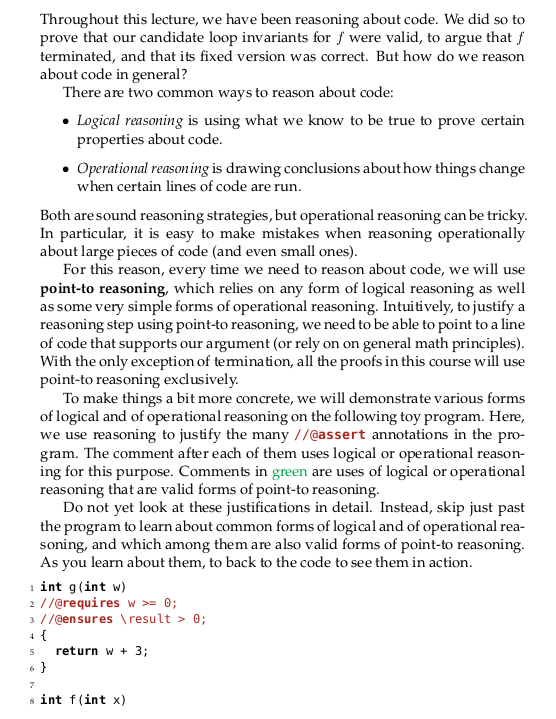
\includegraphics[width=0.8\textwidth]{img/reasoning1.png}
\end{center}
\begin{center}
  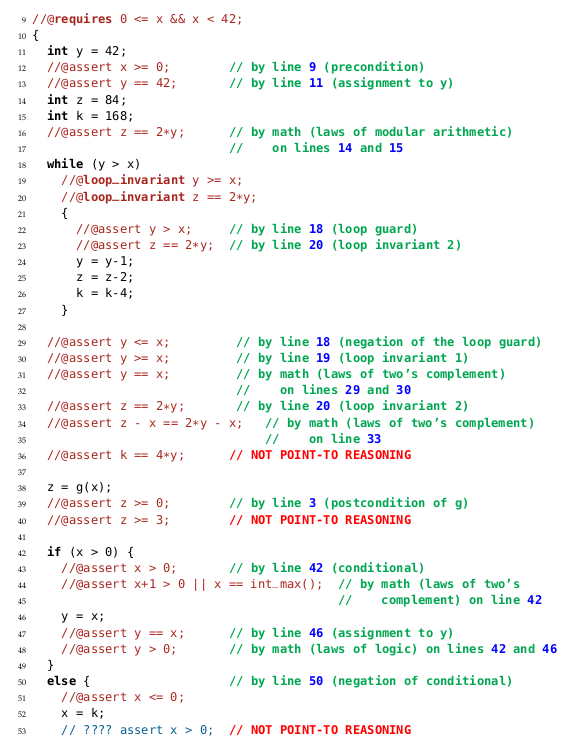
\includegraphics[width=0.8\textwidth]{img/reasoning2.png}
\end{center}
\begin{center}
  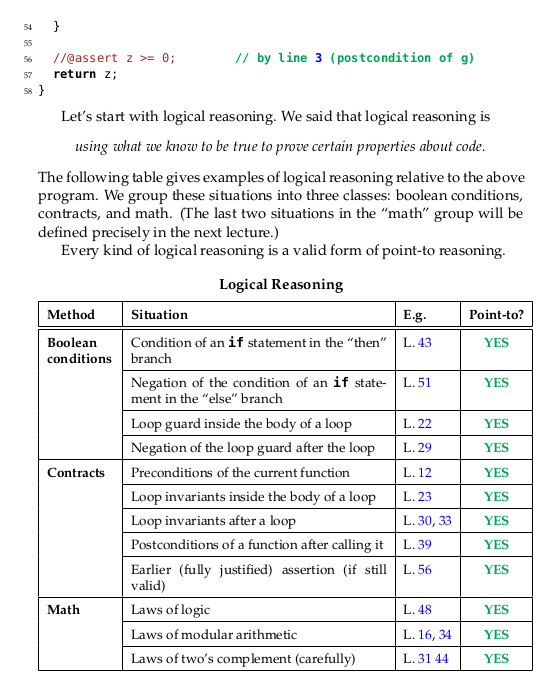
\includegraphics[width=0.8\textwidth]{img/reasoning3.png}
\end{center}
\begin{center}
  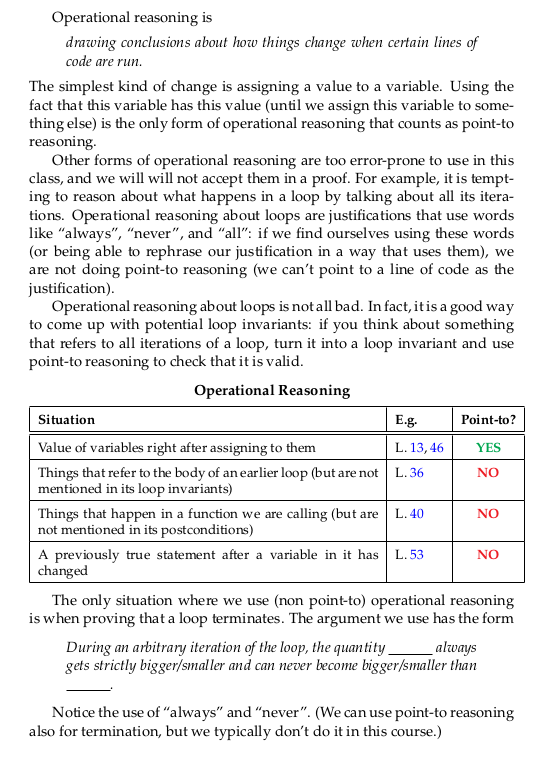
\includegraphics[width=0.8\textwidth]{img/reasoning4.png}
\end{center}


\clearpage
\section{Exercises}
\label{sec:contracts:exercises}

%% \begin{exercise}
%%   After reading
%%   \href{http://www.cs.cmu.edu/~fp/courses/15122-s11/lectures/03-ints.pdf}{Lecture
%%     3} on modular arithmetic go back to the correctness proof in this
%%   lecture and determine if all of the reasoning is valid.  Explain
%%   which steps are questionable and why they are correct or not.  Is
%%   the mystery function correct if all operations (including the
%%   \lstinline'POW' function) are interpreted in modular arithmetic and two's
%%   complement representation of fixed precision integers?
%% \end{exercise}

\begin{flex}
\begin{exercise}[Bad LI]%[\opt{sample solution on page~\pageref{ex:contracts:fast_pow-bad-LI-solved}}]
\label{ex:contracts:fast_pow-bad-LI}
\exerciseTAGS{loop-invariant, testing}
  Find an input for \lstinline'f' that fails our first guess of a loop
  invariant in section~\ref{sec:contracts:loop_invariant}:
  \begin{lstlisting}[language={[C0]C}]
    //@loop_invariant POW(b,e) == POW(x,y);
  \end{lstlisting}
\end{exercise}

\begin{solution}\opt{\textbf{of exercise~\ref{ex:contracts:fast_pow-bad-LI}}}
\label{ex:contracts:fast_pow-bad-LI-solved}
  A call that causes this loop invariant to fail is
  \lstinline'f(2,7)'.
\end{solution}
\end{flex}


\begin{flex}
\begin{exercise}[Another Mystery]%[\opt{sample solution on page~\pageref{ex:contracts:iterated-power-of-2-solved}}]
\label{ex:contracts:iterated-power-of-2}
\exerciseTAGS{correctness, loop-invariant, safety, testing}
Consider the following function:
\begin{lstlisting}[language={[C0]C}]
int foo(int x)
//@requires ___________;
//@ensures ____________;
{
  int p = 0;
  for (int i = 0; i < x; i++)
  //@loop_invariant ____________;
  //@loop_invariant ____________;
  {
     p += POW(2, i);
  }
  return p;
}
\end{lstlisting}
where \lstinline'POW' is the power function defined in this lecture.

After running this function on a few inputs, form a conjecture as to
what it does.  Then, express your conjecture by filling in the
precondition with any constraints on the input \lstinline'x' and the
postcondition with a description of what it computes.  Finally, fill in the
loop invariants that enables you to prove that the safety of every
statement in the loop body and that the postcondition holds
whenever the input satisfies the precondition.
\end{exercise}

\begin{solution}\opt{\textbf{of exercise~\ref{ex:contracts:iterated-power-of-2}}}
\label{ex:contracts:iterated-power-of-2-solved}
This function computes $2^x - 1$ according to the formula
$$
2^x - 1 = \sum_{i=0}^{x-1} 2^i
$$
Here is the resulting code with all contracts filled in:
\begin{lstlisting}[language={[C0]C}]
int foo(int x)
//@requires x >= 0;
//@ensures \result == POW(2,x) - 1;
{
  int p = 0;
  for (int i = 0; i < x; i++)
  //@loop_invariant 0 <= i && i <= x;
  //@loop_invariant p == POW(2,i) - 1;
  {
     p += POW(2, i);
  }
  return p;
}
\end{lstlisting}
\end{solution}
\end{flex}


\begin{flex}
\begin{exercise}[GCD]%[\opt{sample solution on page~\pageref{ex:contracts:gcd-solved}}]
\label{ex:contracts:gcd}
\exerciseTAGS{correctness, loop-invariant, safety}
  The \emph{greatest common divisor} (GCD) of two positive integers
  $a$ and $b$ is the largest integer $d$ such that $a \mathop{\%} d =
  0$ and $b \mathop{\%} d = 0$.  The following function computes the
  GCD of $a$ and $b$ by trying all possible values for $d$ from the
  smallest among $a$ and $b$ down to 1.

\begin{lstlisting}[language={[C0]C}, numbers=left]
int GCD(int a, int b)
//@requires a > 0 && b > 0;
//@ensures \result >= 1;
//@ensures a % \result == 0 && b % \result == 0;
{
  int d = min(a, b);

  while (d > 1)
  //@loop_invariant d >= 1;
  {
    if (a % d == 0 && b % d == 0)
      return d;
    d = d - 1;
  }
  return d;
}
\end{lstlisting}
Using the methodology studied in this chapter and point-to reasoning,
we will show that this code is correct.  Recall that correctness means
that the postconditions must be true for any input that satisfies the
preconditions.  Note that the postconditions say nothing about the
returned value being the \emph{greatest} common divisor of the inputs,
only that it is one of their divisors.

We will proceed in a number of steps.
\begin{enumerate}[label=\alph*]
\item {[INIT]} %
  Show that the loop invariant on line 9 holds
%%   just before checking the loop guard for the very first time.
\item {[PRES]} %
  Show that it is preserved by an arbitrary iteration of the loop.
\item {[EXIT]} %
  Show that the loop invariant and the negation of
  the loop guard imply the postconditions.
\item {[TERM]} %
  Show that the loop terminates.
\item%
  But what if the function exits on line~12?
  Using point-to reasoning, show that the postconditions are satisfied
  also in this case.
\end{enumerate}
\end{exercise}

\begin{solution}\opt{\textbf{of exercise~\ref{ex:contracts:gcd}}}
\label{ex:contracts:gcd-solved}
% \newcommand{\step}[2]{%
% \item\makebox[0.66\linewidth][l]{#1}\hfill%
%      by~\makebox[0.3\linewidth][l]{#2}}

\begin{enumerate}[label=\alph*]
\item {[INIT]} %
  Show that the loop invariant on line 9 holds
  just before checking the loop guard for the very first time.

  We need to show that \lstinline'd >= 1' initially.
  \begin{enumerate}[label=\Alph*.]
  \step{\lstinline'a > 0' and \lstinline'b > 0'}{line~2}
  \step{\lstinline'a >= 1' and \lstinline' b >= 1'}{math on the
    last step}
  \step{\lstinline'd == min(a,b)'}{line~6}
  \step{\lstinline'min(a,b) >= 1'}{math on the last two steps}
  \end{enumerate}

\item {[PRES]} %
  Show that it is preserved by an arbitrary iteration of the loop.

  We need to show that if \lstinline'd >= 1' as we enter an arbitrary
  iteration of the loop, then \lstinline'd` >= 1'.
  \begin{enumerate}[label=\Alph*.]
  \step{\lstinline'd > 1'}{line~8}
  \step{\lstinline'd` == d-1'}{line~13}
  \step{\lstinline'd` >= 1'}{math on the last two steps}
  \end{enumerate}
  In this proof, we did not make use of the assumption that %
  \lstinline'd >= 1'.  This is not typical as most proofs of
  preservation rely critically on their assumption.

\item {[EXIT]} %
  Show that the loop invariant and the negation of the loop guard
  imply the postconditions.

  We need to show that \lstinline'd >= 1' and %
  \lstinline'a % d == 0 && b % d == 0' hold on
  line~15.

  \begin{enumerate}[label=\Alph*.]
  \step{\lstinline'd >= 1'}{line~9}
  \step{\lstinline'd <= 1'}{line~8}
  \step{\lstinline'd == 1'}{math on the last two steps}
  \step{$n \mathop{\%} 1 = 0$ for any $n > 0$}{math}
  \end{enumerate}
  This proof suggest simplifying line~15 into
  \lstinline'return 1', since this is the only possible value that
  \lstinline'd' can assume.

\item {[TERM]} %
  Show that the loop terminates.

  During an arbitrary iteration of the loop, the quantity
  \lstinline'd' strictly decreases and can never get smaller than 1.

\item%
  But what if the function exits on line~12?
  Using point-to reasoning, show that the postconditions are satisfied
  also in this case.

  We need to show that \lstinline'd >= 1' and %
  \lstinline'a % d == 0 && b % d == 0' hold on
  line~12.

  \begin{enumerate}[label=\Alph*.]
  \step{\lstinline'd >= 1'}{line~9}
  \step{\lstinline'a \% d == 0 && b \% d == 0'}{line~11}
  \end{enumerate}
\end{enumerate}
\end{solution}
\end{flex}


\begin{flex}
\begin{exercise}[Euclid]%[\opt{sample solution on page~\pageref{ex:contracts:euclid-solved}}]
\label{ex:contracts:euclid}
\exerciseTAGS{correctness, loop-invariant, safety}
  \emph{Euclid's algorithm} computes the greatest common divisor of two
  numbers, a problem we already explored in Exercise~\ref{ex:contracts:gcd}.  It
  is often more efficient, but not as obviously correct.  In this
  exercise, we will use the methodology developed in his chapter to
  convince ourselves (and others) of its correctness.

This code uses the function \lstinline'GCD' from Exercise~\ref{ex:contracts:gcd}
as a specification function.
\begin{lstlisting}[language={[C0]C}, numbers=left]
int euclid(int a, int b)
//@requires a > 0 && b > 0;
//@ensures \result == GCD(a, b);
{
  int x = a;
  int y = b;

  while (x != y)
  //@loop_invariant x > 0 && y > 0;
  //@loop_invariant GCD(x, y) == GCD(a, b);
  {
    if (x > y)
      x = x - y;
    else
      y = y - x;
  }
  //@assert x == y;
  return x;
}
\end{lstlisting}

We will follow the usual steps to prove correctness, plus one, to ensure
safety.
\begin{enumerate}[label=\alph*]
\item%
  Show that the calls to \lstinline'GCD' on line~10
  are safe.
\item {[INIT]} %
  Show that the loop invariants on
  lines~9--10 hold just before
  checking the loop guard for the very first time.
\item {[PRES]} %
  Show that they are preserved by an arbitrary iteration of the loop.
\item {[EXIT]} %
  Show that the loop invariants and the negation of
  the loop guard imply the postconditions.
\item {[TERM]} %
  Show that the loop terminates.
\end{enumerate}
\end{exercise}

\begin{solution}\opt{\textbf{of exercise~\ref{ex:contracts:euclid}}}
\label{ex:contracts:euclid-solved}
% \newcommand{\step}[2]{%
% \item\makebox[0.66\linewidth][l]{#1}\hfill%
%      by~\makebox[0.3\linewidth][l]{#2}}

\begin{enumerate}[label=\alph*)]
\item%
  Show that the calls to \lstinline'GCD' on line~10
  are safe.

  We need to show that the preconditions of both calls to
  \lstinline'GCD' are satisfied, i.e., %
  that \lstinline'x > 0 && y > 0' for \lstinline'GCD(x,y)'
  and \lstinline'a > 0 && b > 0' for \lstinline'GCD(a,b)'.

  \begin{enumerate}[label=\Alph*.]
  \step{\lstinline'x > 0 && y > 0'}{line~9}
  \step{\lstinline'a > 0 && b > 0'}{line~2}
  \end{enumerate}


\item {[INIT]} %
  Show that the loop invariants on
  lines~9--10 hold just before
  checking the loop guard for the very first time.

  We need to show that \lstinline'x > 0 && y > 0' and that
  \lstinline'GCD(x,y) == GCD(a,b)'. initially.
  \begin{enumerate}[label=\Alph*.]
  \step{\lstinline'x = a'}{line~5}
  \step{\lstinline'y = b'}{line~6}
  \step{\lstinline'a > 0 && b > 0'}{line~2}
  \step{\lstinline'GCD(a,b) == GCD(a,b)'}{math on the first two steps}
  \end{enumerate}

\item {[PRES]} %
  Show that they are preserved by an arbitrary iteration of the loop.

  Assuming that \lstinline'x > 0 && y > 0' and that %
  \lstinline'GCD(x,y) == GCD(a,b)', we need to show that
  \lstinline'x` > 0 && y` > 0' and %
  \lstinline'GCD(x`,y`) == GCD(a,b)'.

  We need to consider two cases depending on whether
  \lstinline'x > y' or \lstinline'x < y'.

  Assume that \lstinline'x > y':
  \begin{enumerate}[label=\Alph*.]
    \step{\lstinline'x > y'}{assumption}
    \step{\lstinline'x - y > 0'}{math on the last step}
    \step{\lstinline'x` == x - y'}{line~13}
    \step{\lstinline'x` > 0'}{the last two steps}
    \step{\lstinline'y` > 0'}{line~9 and
      \lstinline'y' is unchanged}
    \step{$\mathit{GCD}(n,m) == GCD(n-m,m)$}{math}
    \step{\lstinline'GCD(x-y,y) == GCD(a,b)'}{math and line 9}
  \end{enumerate}

  Assume that \lstinline'x < y': the proof is similar.

\item {[EXIT]} %
  Show that the loop invariants and the negation of
  the loop guard imply the postconditions.

  \begin{enumerate}[label=\Alph*.]
    \step{\lstinline'x == y'}{line~8}
    \step{\lstinline'GCD(x,x) == GCD(a,b)'}{line~10}
    \step{$\mathit{GCD}(n,n) == n$ for any $n > 0$}{math}
    \step{\lstinline'x == GCD(a,b)'}{math on the last two steps}
  \end{enumerate}
  Step (A) is also noted as an assertion on line~17.


\item {[TERM]} %
  Show that the loop terminates.

  During an arbitrary iteration of the loop, the quantity %
  \lstinline'x + y' is strictly decreasing and can never get smaller
  than 2.  The fact that \lstinline'x + y' is strictly decreasing
  relies on the fact that \lstinline'x' and \lstinline'y' are positive
  by the second loop invariant (line~10):
  if \lstinline'x > y' the quantity \lstinline'x + y' is updated to
  \lstinline'x', and otherwise it is updated to \lstinline'y', either
  of which is strictly smaller than \lstinline'x + y'.  The lower
  bound (2) is a consequence of the first loop invariant.
\end{enumerate}

\end{solution}
\end{flex}

\printsolutions
% \clearpage
% \bibliographystyle{alpha}
% \bibliography{modal}

% \cleardoublepage
